\documentclass[11pt,a4paper]{report}
\usepackage[textwidth=37em,vmargin=30mm]{geometry}
\usepackage{calc,xunicode,amsmath,amssymb,paralist,enumitem,tabu,booktabs,datetime2,xeCJK,xeCJKfntef,listings}
\usepackage{tocloft,fancyhdr,tcolorbox,xcolor,graphicx,eso-pic,xltxtra,xelatexemoji}

\newcommand{\envyear}[0]{2025}
\newcommand{\envdatestr}[0]{2025-06-22}
\newcommand{\envfinaldir}[0]{webdb/2025/20250622/final}

\usepackage[hidelinks]{hyperref}
\hypersetup{
    colorlinks=false,
    pdfpagemode=FullScreen,
    pdftitle={Web Digest - \envdatestr}
}

\setlength{\cftbeforechapskip}{10pt}
\renewcommand{\cftchapfont}{\rmfamily\bfseries\large\raggedright}
\setlength{\cftbeforesecskip}{2pt}
\renewcommand{\cftsecfont}{\sffamily\small\raggedright}

\setdefaultleftmargin{2em}{2em}{1em}{1em}{1em}{1em}

\usepackage{xeCJK,xeCJKfntef}
\xeCJKsetup{PunctStyle=plain,RubberPunctSkip=false,CJKglue=\strut\hskip 0pt plus 0.1em minus 0.05em,CJKecglue=\strut\hskip 0.22em plus 0.2em}
\XeTeXlinebreaklocale "zh"
\XeTeXlinebreakskip = 0pt


\setmainfont{Brygada 1918}
\setromanfont{Brygada 1918}
\setsansfont{IBM Plex Sans}
\setmonofont{JetBrains Mono NL}
\setCJKmainfont{Noto Serif CJK SC}
\setCJKromanfont{Noto Serif CJK SC}
\setCJKsansfont{Noto Sans CJK SC}
\setCJKmonofont{Noto Sans CJK SC}

\setlength{\parindent}{0pt}
\setlength{\parskip}{8pt}
\linespread{1.15}

\lstset{
	basicstyle=\ttfamily\footnotesize,
	numbersep=5pt,
	backgroundcolor=\color{black!5},
	showspaces=false,
	showstringspaces=false,
	showtabs=false,
	tabsize=2,
	captionpos=b,
	breaklines=true,
	breakatwhitespace=true,
	breakautoindent=true,
	linewidth=\textwidth
}






\newcommand{\coverpic}[2]{
    % argv: itemurl, authorname
    Cover photo by #2~~(\href{#1}{#1})
}
\newcommand{\makeheader}[0]{
    \begin{titlepage}
        % \newgeometry{hmargin=15mm,tmargin=21mm,bmargin=12mm}
        \begin{center}
            
            \rmfamily\scshape
            \fontspec{BaskervilleF}
            \fontspec{Old Standard}
            \fontsize{59pt}{70pt}\selectfont
            WEB\hfill DIGEST
            
            \vfill
            % \vskip 30pt
            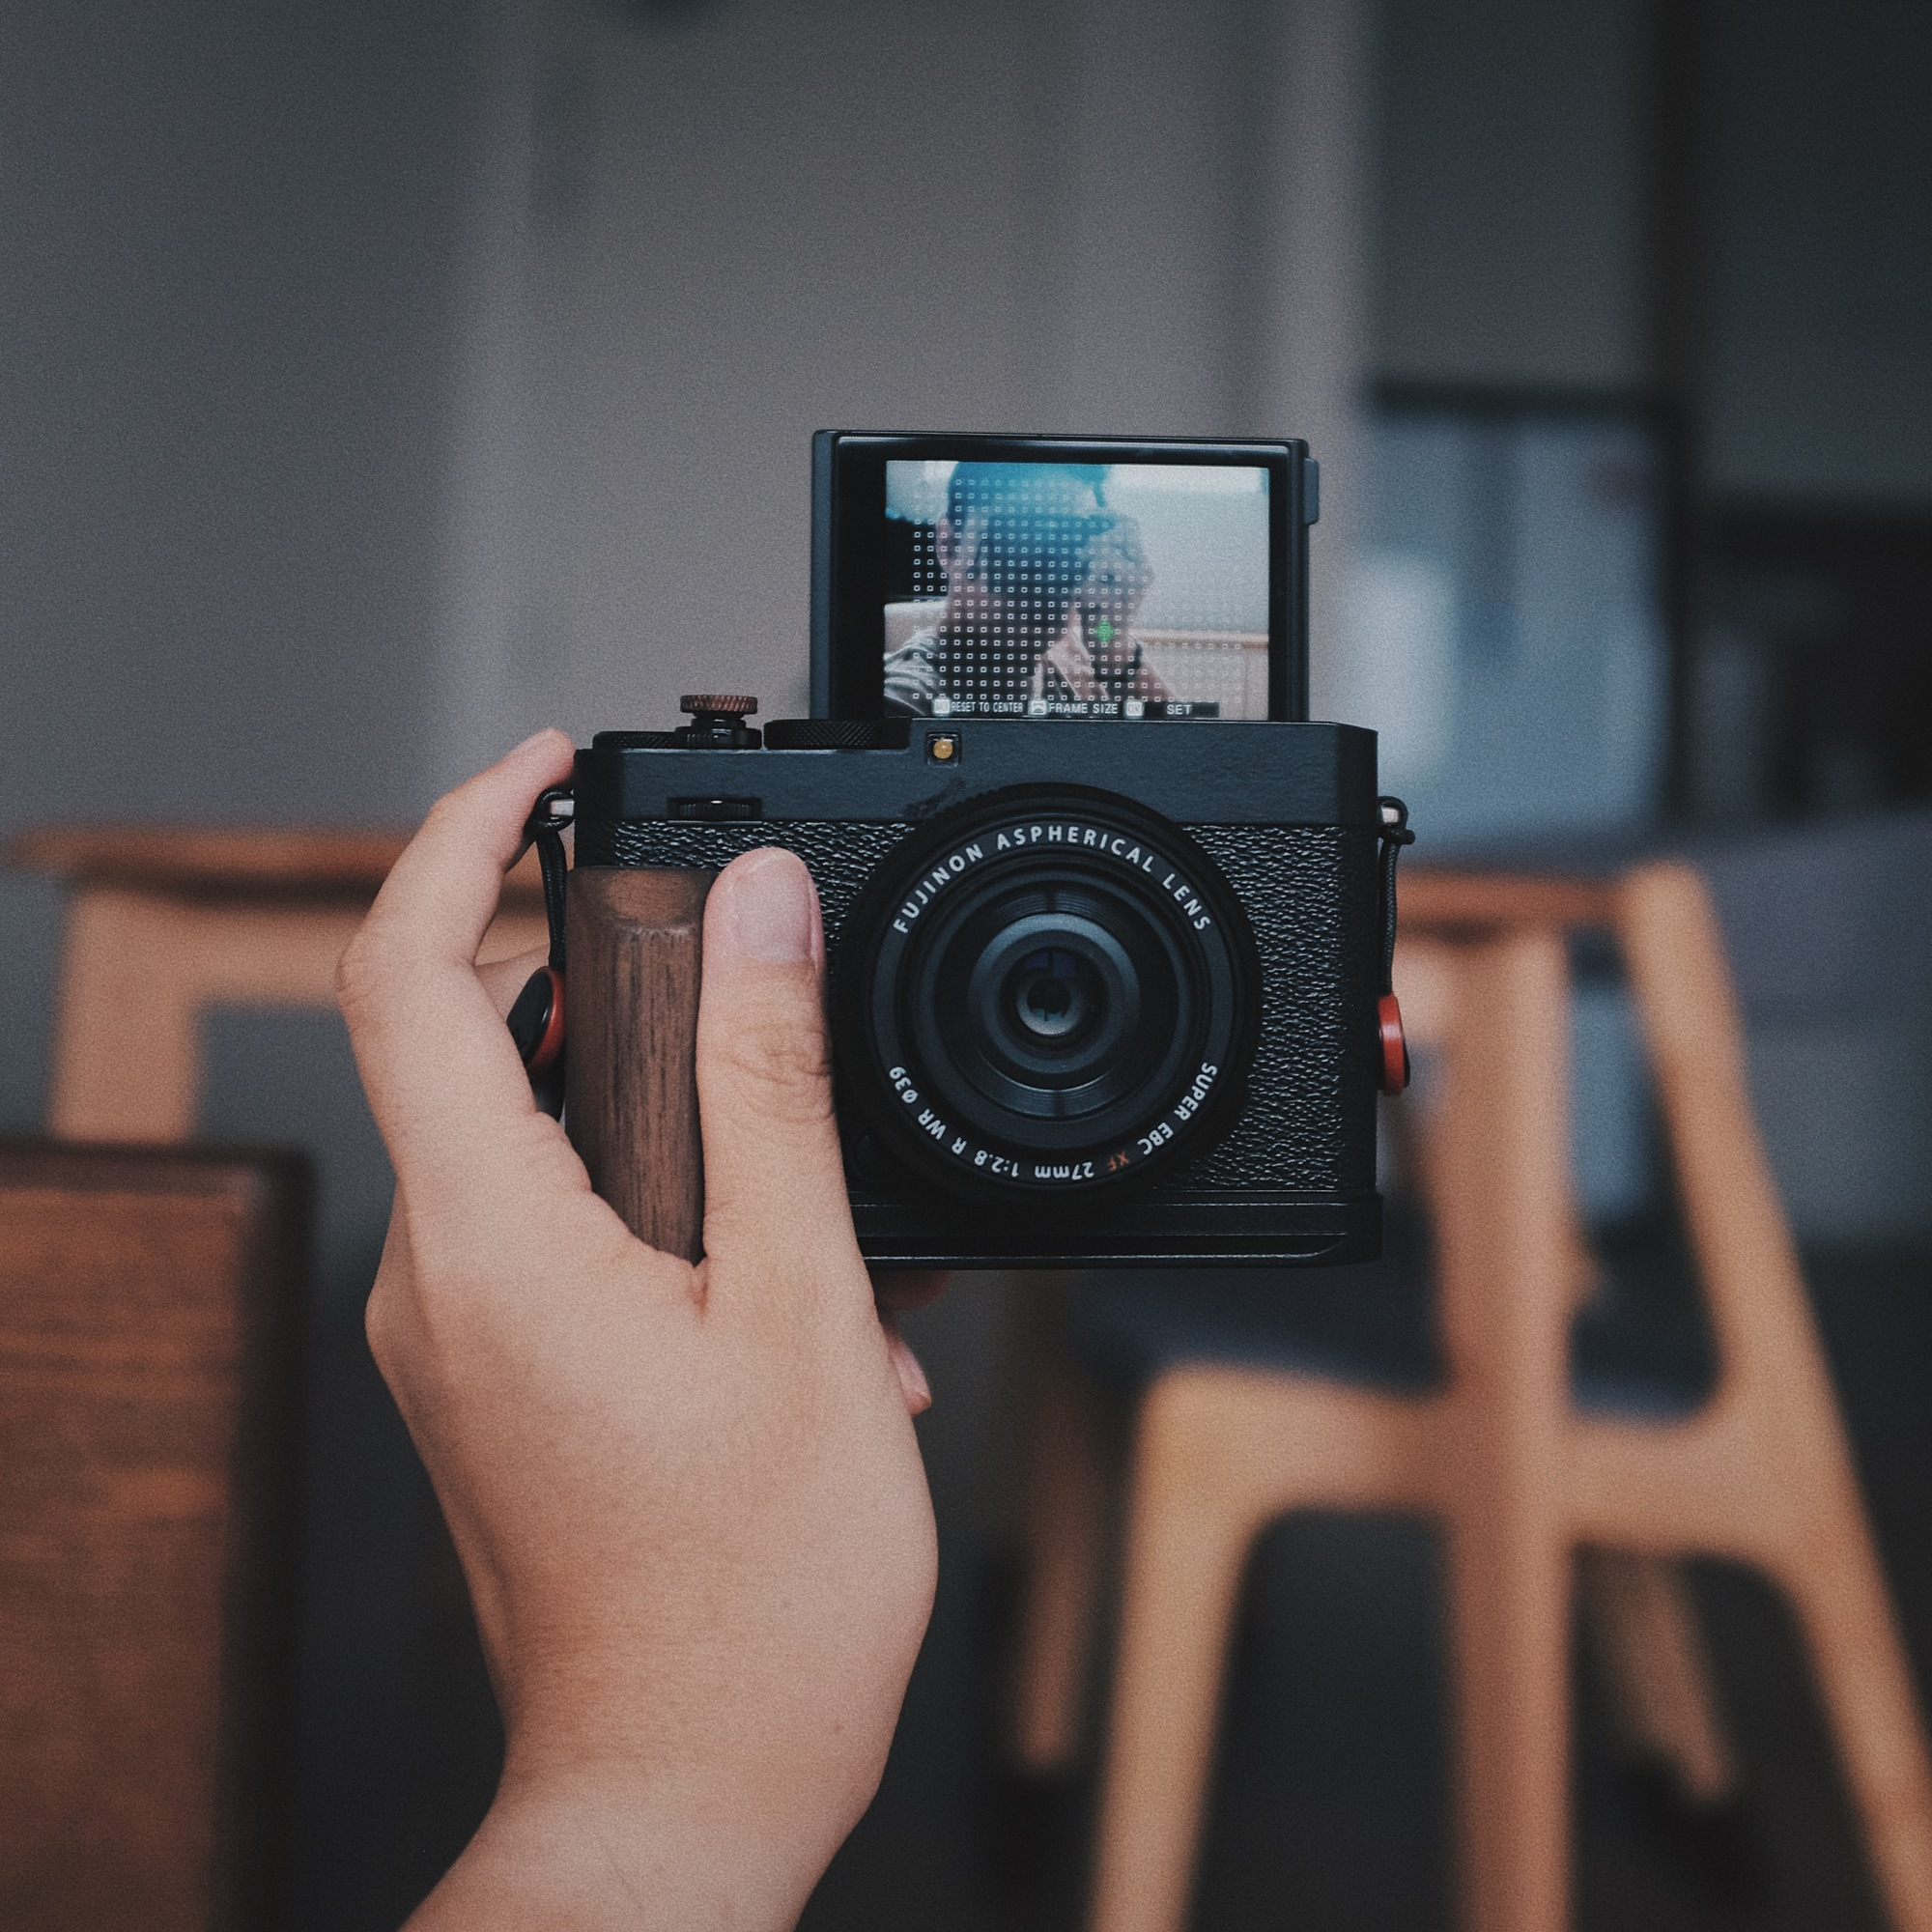
\includegraphics[width=\linewidth]{\envfinaldir/coverpic-prod.jpg}\par
            % \vskip 30pt
            \vfill

            \normalsize\rmfamily\scshape
            \copyright{} The Web Digest Project \hfill\large \envdatestr
        \end{center}
    \end{titlepage}
    % \restoregeometry
}
\newcommand{\simplehref}[1]{%
    \textcolor{blue!80!green}{\href{#1}{#1}}%
}
\renewcommand{\contentsname}{\center\Huge\sffamily\bfseries Contents\par\vskip 20pt}
\newcounter{ipartcounter}
\setcounter{ipartcounter}{0}
\newcommand{\ipart}[1]{
    % \vskip 20pt
    \clearpage
    \stepcounter{ipartcounter}
    \phantomsection
    \addcontentsline{toc}{chapter}{#1}
    % \begin{center}
    %     \Huge
    %     \sffamily\bfseries
    %     #1
    % \end{center}
    % \vskip 20pt plus 7pt
}
\newcounter{ichaptercounter}
\setcounter{ichaptercounter}{0}
\newcommand{\ichapter}[1]{
    % \vskip 20pt
    \clearpage
    \stepcounter{ichaptercounter}
    \phantomsection
    \addcontentsline{toc}{section}{\numberline{\arabic{ichaptercounter}}#1}
    \begin{center}
        \Huge
        \sffamily\bfseries
        #1
    \end{center}
    \vskip 20pt plus 7pt
}
\newcommand{\entrytitlefont}[1]{\subsection*{\raggedright\Large\sffamily\bfseries#1}}
\newcommand{\entryitemGeneric}[2]{
    % argv: title, url
    \parbox{\linewidth}{
        \entrytitlefont{#1}\par\vskip 5pt
        \footnotesize\ttfamily\mdseries
        \simplehref{#2}
    }\vskip 11pt plus 11pt minus 1pt
}
\newcommand{\entryitemGithub}[3]{
    % argv: title, url, desc
    \parbox{\linewidth}{
        \entrytitlefont{#1}\par\vskip 5pt
        \footnotesize\ttfamily\mdseries
        \simplehref{#2}\par\vskip 5pt
        \small\rmfamily\mdseries#3
    }\vskip 11pt plus 11pt minus 1pt
}
\newcommand{\entryitemAp}[3]{
    % argv: title, url, desc
    \parbox{\linewidth}{
        \entrytitlefont{#1}\par\vskip 5pt
        \footnotesize\ttfamily\mdseries
        \simplehref{#2}\par\vskip 5pt
        \small\rmfamily\mdseries#3
    }\vskip 11pt plus 11pt minus 1pt
}
\newcommand{\entryitemHackernews}[3]{
    % argv: title, hnurl, rawurl
    % \parbox{\linewidth}{
    %     \entrytitlefont{#1}\par\vskip 5pt
    %     \footnotesize\ttfamily\mdseries
    %     \simplehref{#3}\par
    %     \textcolor{black!50}{\href{#2}{#2}}
    % }\vskip 11pt plus 11pt minus 1pt
    \begin{minipage}{\linewidth}
            \entrytitlefont{#1}\par\vskip 5pt
            \footnotesize\ttfamily\mdseries
            \simplehref{#3}\par
            \textcolor{black!50}{\href{#2}{#2}}
    \end{minipage}\par\vskip 11pt plus 11pt minus 1pt
}







\begin{document}

\makeheader

\tableofcontents\clearpage




\ipart{Developers}
\ichapter{Hacker News}
\entryitemTwoLinks{Tell HN: Beware confidentiality agreements that act as lifetime non competes}{https://news.ycombinator.com/item?id=44338562}{https://news.ycombinator.com/item?id=44338562}

\entryitemTwoLinks{US Congress is making more than 250M acres of public lands available for sale}{https://news.ycombinator.com/item?id=44338122}{https://www.wilderness.org/articles/blog/congress-making-more-250-million-acres-public-lands-available-sale}

\entryitemTwoLinks{Microsoft suspended the email account of an ICC prosecutor at The Hague}{https://news.ycombinator.com/item?id=44336915}{https://www.nytimes.com/2025/06/20/technology/us-tech-europe-microsoft-trump-icc.html}

\entryitemTwoLinks{Scaling our observability platform by embracing wide events and replacing OTel}{https://news.ycombinator.com/item?id=44336015}{https://clickhouse.com/blog/scaling-observability-beyond-100pb-wide-events-replacing-otel}

\entryitemTwoLinks{We moved from AWS to Hetzner, saved 90\%, kept ISO 27001 with Ansible}{https://news.ycombinator.com/item?id=44335920}{https://medium.com/@accounts\_73078/goodbye-aws-how-we-kept-iso-27001-slashed-costs-by-90-914ccb4b89fc}

\entryitemTwoLinks{Cosmoe: BeOS Class Library on Top of Wayland}{https://news.ycombinator.com/item?id=44335907}{https://cosmoe.org/index.html}

\entryitemTwoLinks{uBlock Origin Lite Beta for Safari iOS}{https://news.ycombinator.com/item?id=44335664}{https://testflight.apple.com/join/JjTcThrV}

\entryitemTwoLinks{'Gwada negative': French scientists find new blood type in woman}{https://news.ycombinator.com/item?id=44335517}{https://www.lemonde.fr/en/science/article/2025/06/21/gwada-negative-french-scientists-find-new-blood-type-in-woman\_6742577\_10.html}

\entryitemTwoLinks{Delta Chat is a decentralized and secure messenger app}{https://news.ycombinator.com/item?id=44335065}{https://delta.chat/en/}

\entryitemTwoLinks{Sega mistakenly reveals sales numbers of popular games}{https://news.ycombinator.com/item?id=44335038}{https://www.gematsu.com/2025/06/sega-mistakenly-reveals-sales-numbers-for-like-a-dragon-infinite-wealth-persona-3-reload-shin-megami-tensei-v-and-more}

\entryitemTwoLinks{Signal – An Ethical Replacement for WhatsApp}{https://news.ycombinator.com/item?id=44334743}{https://greenstarsproject.org/2025/06/15/signal-an-ethical-replacement-for-whatsapp/}

\entryitemTwoLinks{Samsung embeds IronSource spyware app on phones across WANA}{https://news.ycombinator.com/item?id=44334167}{https://smex.org/open-letter-to-samsung-end-forced-israeli-app-installations-in-the-wana-region/}

\entryitemTwoLinks{Tiny Undervalued Hardware Companions (2024)}{https://news.ycombinator.com/item?id=44333960}{https://vermaden.wordpress.com/2024/03/21/tiny-undervalued-hardware-companions/}

\entryitemTwoLinks{Learn you Galois fields for great good (2023)}{https://news.ycombinator.com/item?id=44333388}{https://xorvoid.com/galois\_fields\_for\_great\_good\_00.html}

\entryitemTwoLinks{Plastic bag bans and fees reduce harmful bag litter on shorelines}{https://news.ycombinator.com/item?id=44333187}{https://www.science.org/doi/10.1126/science.adp9274}

\entryitemTwoLinks{AbsenceBench: Language models can't tell what's missing}{https://news.ycombinator.com/item?id=44332699}{https://arxiv.org/abs/2506.11440}

\entryitemTwoLinks{AMD's Freshly-Baked MI350: An Interview with the Chief Architect}{https://news.ycombinator.com/item?id=44332221}{https://chipsandcheese.com/p/amds-freshly-baked-mi350-an-interview}

\entryitemTwoLinks{Wiki Radio: The thrilling sound of random Wikipedia}{https://news.ycombinator.com/item?id=44332170}{https://www.monkeon.co.uk/wikiradio/}

\entryitemTwoLinks{BYD begins testing solid-state EV batteries in the Seal}{https://news.ycombinator.com/item?id=44331898}{https://electrek.co/2025/06/20/byd-tests-solid-state-batteries-seal-ev-with-1000-miles-range/}

\entryitemTwoLinks{Show HN: Inspect and extract files from MSI installers directly in your browser}{https://news.ycombinator.com/item?id=44331518}{https://pymsi.readthedocs.io/en/latest/msi\_viewer.html}


\ipart{Developers~~~~(zh-Hans)}
\ichapter{Solidot}
\entryitemGeneric{\hskip 0pt{}3 亿年前的全球暖化}{https://www.solidot.org/story?sid=81615}

\entryitemGeneric{\hskip 0pt{}智能手机是人类的寄生物}{https://www.solidot.org/story?sid=81614}

\entryitemGeneric{\hskip 0pt{}中国科学家培育出有两个父亲的健康小鼠}{https://www.solidot.org/story?sid=81613}

\entryitemGeneric{\hskip 0pt{}公民社会组织呼吁打破科技寡头对数字世界的控制}{https://www.solidot.org/story?sid=81612}

\entryitemGeneric{\hskip 0pt{}在试验之后澳大利亚准备实施儿童社媒禁令}{https://www.solidot.org/story?sid=81610}

\entryitemGeneric{\hskip 0pt{}苹果无意统一桌面和平板的操作系统}{https://www.solidot.org/story?sid=81609}

\entryitemGeneric{\hskip 0pt{}Jolla 放弃手机软件更新的付费订阅制}{https://www.solidot.org/story?sid=81608}

\entryitemGeneric{\hskip 0pt{}过去两个月 iPhone 销量同比增长 15\%}{https://www.solidot.org/story?sid=81607}

\entryitemGeneric{\hskip 0pt{}塑料袋管制政策显著减少美国海岸线的塑料垃圾}{https://www.solidot.org/story?sid=81606}

\entryitemGeneric{\hskip 0pt{}恐龙求偶时可能也会跳舞}{https://www.solidot.org/story?sid=81605}

\entryitemGeneric{\hskip 0pt{}Switch 2 在电商平台热销}{https://www.solidot.org/story?sid=81604}

\entryitemGeneric{\hskip 0pt{}骗子使用 Google 广告在苹果微软网站注入假的技术支持电话号码}{https://www.solidot.org/story?sid=81603}

\entryitemGeneric{\hskip 0pt{}Kali Linux 2025.2 释出}{https://www.solidot.org/story?sid=81602}

\entryitemGeneric{\hskip 0pt{}《自然》期刊公开所有论文的审稿人评论}{https://www.solidot.org/story?sid=81601}

\entryitemGeneric{\hskip 0pt{}城市人造光源的规模有多大}{https://www.solidot.org/story?sid=81600}

\entryitemGeneric{\hskip 0pt{}SpaceX 的 Starship 36 在静态点火测试中爆炸}{https://www.solidot.org/story?sid=81599}

\entryitemGeneric{\hskip 0pt{}石油巨头面临首宗气候死亡诉讼}{https://www.solidot.org/story?sid=81598}

\entryitemGeneric{\hskip 0pt{}秸秆覆盖大幅增加竹林土壤碳排放}{https://www.solidot.org/story?sid=81597}

\entryitemGeneric{\hskip 0pt{}媒体竞争如何驱动虚假信息传播}{https://www.solidot.org/story?sid=81596}

\entryitemGeneric{\hskip 0pt{}美国新签证规定要求留学生将社媒账号设为公开}{https://www.solidot.org/story?sid=81595}\ichapter{V2EX}
\entryitemGeneric{\hskip 0pt{}[瑞典] 钥匙掉进了电梯缝里}{https://www.v2ex.com/t/1140189}

\entryitemGeneric{\hskip 0pt{}[English] 作为一个 i 人如何快速提高英语水平}{https://www.v2ex.com/t/1140188}

\entryitemGeneric{\hskip 0pt{}[宽带症候群] 江苏联通有人获取到 116.147.71.0/24 的公网 ip 么?}{https://www.v2ex.com/t/1140187}

\entryitemGeneric{\hskip 0pt{}[Android] 有安卓系统的智能手表推荐吗?需要可插卡,可独立电话,}{https://www.v2ex.com/t/1140186}

\entryitemGeneric{\hskip 0pt{}[酷工作] [远程 前端/后端]初创出海 AI 产品公司,寻靠谱前端,后端工程师}{https://www.v2ex.com/t/1140183}

\entryitemGeneric{\hskip 0pt{}[职场话题] offer 有时间差,怎么办}{https://www.v2ex.com/t/1140182}

\entryitemGeneric{\hskip 0pt{}[酷工作] 上海张江: AI 大模型应用 Leader, 100 万}{https://www.v2ex.com/t/1140180}

\entryitemGeneric{\hskip 0pt{}[Android] 安卓软件开发中,如何获取摄像头的最高规格数据?}{https://www.v2ex.com/t/1140178}

\entryitemGeneric{\hskip 0pt{}[问与答] v 站的前端大佬们,紧急求助!}{https://www.v2ex.com/t/1140177}

\entryitemGeneric{\hskip 0pt{}[分享创造] Web 搜索 MCP 启动!}{https://www.v2ex.com/t/1140175}

\entryitemGeneric{\hskip 0pt{}[分享发现] [免费领取] 微信提现额度}{https://www.v2ex.com/t/1140174}

\entryitemGeneric{\hskip 0pt{}[生活] 新房要买电器了,想问问大家有什么好用的电器推荐}{https://www.v2ex.com/t/1140173}

\entryitemGeneric{\hskip 0pt{}[游戏开发] 个人开发者想试水一下 2D 游戏开发,应该怎么选框架?}{https://www.v2ex.com/t/1140172}

\entryitemGeneric{\hskip 0pt{}[宽带症候群] 双栈公网,不知道还能用多久}{https://www.v2ex.com/t/1140170}

\entryitemGeneric{\hskip 0pt{}[NAS] Nas 星际蜗牛 c 款请教几个问题}{https://www.v2ex.com/t/1140169}

\entryitemGeneric{\hskip 0pt{}[问与答] 抖音橱窗 商品图片 搞成这个样子真的不违规吗?? 谁能受得了?}{https://www.v2ex.com/t/1140167}

\entryitemGeneric{\hskip 0pt{}[iOS] iPhone 16, 更新 iOS 18.5(18.4?)后锁屏右滑无法快捷录制}{https://www.v2ex.com/t/1140166}

\entryitemGeneric{\hskip 0pt{}[全球工单系统] 飞书 AI 划词工具自动开启,你礼貌么}{https://www.v2ex.com/t/1140163}

\entryitemGeneric{\hskip 0pt{}[程序员] 做 app 里的 app,我算不上独立开发}{https://www.v2ex.com/t/1140161}

\entryitemGeneric{\hskip 0pt{}[宽带症候群] 一般上行流量要到多少运营商才会搞小动作?}{https://www.v2ex.com/t/1140160}

\entryitemGeneric{\hskip 0pt{}[微信] 微信给别人打电话时的铃声怎么关?}{https://www.v2ex.com/t/1140159}

\entryitemGeneric{\hskip 0pt{}[分享创造] 腾讯云国际的 EdgeOne CDN 用上了,欢迎大家测试速度}{https://www.v2ex.com/t/1140158}

\entryitemGeneric{\hskip 0pt{}[问与答] 5220 年了,有老板先享受 fydetab duo 了吗? 四不像 还是 六边形战士?}{https://www.v2ex.com/t/1140157}

\entryitemGeneric{\hskip 0pt{}[Local LLM] 有个大模型相关的副业想法,大家帮忙看看有没有需求}{https://www.v2ex.com/t/1140155}

\entryitemGeneric{\hskip 0pt{}[问与答] 3km 城市范围内如何物联网通讯?}{https://www.v2ex.com/t/1140154}

\entryitemGeneric{\hskip 0pt{}[分享发现] AI 编程上线第 11 个网站: Veozon AI 视频创作工具站}{https://www.v2ex.com/t/1140153}

\entryitemGeneric{\hskip 0pt{}[游戏] 33 号远征队 真是个好游戏}{https://www.v2ex.com/t/1140151}

\entryitemGeneric{\hskip 0pt{}[分享创造] 做了一款跨平台电子书阅读器 Reeden}{https://www.v2ex.com/t/1140150}

\entryitemGeneric{\hskip 0pt{}[生活] 有 v 友知道这四五年间的希尔顿会员条款变化吗}{https://www.v2ex.com/t/1140149}

\entryitemGeneric{\hskip 0pt{}[微信] 微信多久不能全选复制了}{https://www.v2ex.com/t/1140148}

\entryitemGeneric{\hskip 0pt{}[macOS] 如何设置程序坞能像 PC 一样点击图标即可最小化/恢复窗口}{https://www.v2ex.com/t/1140147}

\entryitemGeneric{\hskip 0pt{}[Android] 一加 13 顶配,过来人指点一下安卓要怎么高质量体验?}{https://www.v2ex.com/t/1140146}

\entryitemGeneric{\hskip 0pt{}[Apple] 现在苹果笔记本的产能都在越南了?}{https://www.v2ex.com/t/1140145}

\entryitemGeneric{\hskip 0pt{}[Go 编程语言] 最近不知道为什么编译速度超级慢,最后发现是 MicrosoftPCManager}{https://www.v2ex.com/t/1140144}

\entryitemGeneric{\hskip 0pt{}[推广] HornetPay 虚拟 visa 卡, 免费 200 张, 先到先得}{https://www.v2ex.com/t/1140143}

\entryitemGeneric{\hskip 0pt{}[分享发现] 使用 github action 编译自定义 rustdesk 客户端指南(内置服务器信息、内置固定密码、内置自定义 api 服务器)}{https://www.v2ex.com/t/1140142}

\entryitemGeneric{\hskip 0pt{}[生活] 有没有好用的扫地机器人推荐,要求简单易用,适合中老年人使用}{https://www.v2ex.com/t/1140139}

\entryitemGeneric{\hskip 0pt{}[VPS] 甲骨文免费 VPS 速率降太多了,现在闲时也只有 46Mbps}{https://www.v2ex.com/t/1140138}

\entryitemGeneric{\hskip 0pt{}[酷工作] 深圳 龙华 香港公司招聘 AIagent 运营工程师}{https://www.v2ex.com/t/1140137}

\entryitemGeneric{\hskip 0pt{}[问与答] 折叠屏手机 可以有隐私贴膜吗?}{https://www.v2ex.com/t/1140135}

\entryitemGeneric{\hskip 0pt{}[宽带症候群] 用腾讯云免费 edgeone 实现加速、免端口、双栈访问家里服务}{https://www.v2ex.com/t/1140134}

\entryitemGeneric{\hskip 0pt{}[分享创造] [热门动画] 极简模式上线,一图流展示,方便分享}{https://www.v2ex.com/t/1140132}

\entryitemGeneric{\hskip 0pt{}[问与答] 用电信宽带还是用随身 wifi 或者有更便宜的?}{https://www.v2ex.com/t/1140130}

\entryitemGeneric{\hskip 0pt{}[问与答] 求一个替代 G304 的无线鼠标}{https://www.v2ex.com/t/1140129}

\entryitemGeneric{\hskip 0pt{}[Podcast] [分享] 发现一个能让英文播客``说中文''的工具,没有机味,简直完美还原! Naval, HubermanLab, A16z, Lennys 都可以直接中文来听}{https://www.v2ex.com/t/1140128}

\entryitemGeneric{\hskip 0pt{}[旅行] 普吉岛旅游 指南 求请教}{https://www.v2ex.com/t/1140127}

\entryitemGeneric{\hskip 0pt{}[求职] 毕业了,在找工作了,各位前辈能不能在简历或未来学习发展上给点建议}{https://www.v2ex.com/t/1140126}

\entryitemGeneric{\hskip 0pt{}[分享发现] 分享一个恶趣味的网站}{https://www.v2ex.com/t/1140125}

\entryitemGeneric{\hskip 0pt{}[问与答] 有没有什么真正可用的旅游规划的 AI 啊?}{https://www.v2ex.com/t/1140124}

\entryitemGeneric{\hskip 0pt{}[怀旧游戏] v 友 有没有玩过尼彩手机的游戏, 《孤岛》《众神之战》}{https://www.v2ex.com/t/1140123}


\ipart{Generic News}
\ichapter{联合早报}
\entryitemWithDescription{杨丹旭:关税战中找定力}{https://www.zaobao.com/news/china/story20250617-6814940}{中美伦敦经贸磋商后,美国媒体彭博社发表了一篇评论文章,概括中美对待这场贸易争端截然不同的两种思维:美国领导人急于出成果,而中国领导人专注打长线战。 评论指出,中美伦敦经贸磋商后,美国总统特朗普对谈判结果大加赞赏,不仅在社交媒体上宣布,已与中国达成``协议'',来自中国的关键磁铁将恢复供应,美国也承诺会放宽对中国学生的签证限制……}

\entryitemWithDescription{中国5月消费显著回升达6.4\%成经济亮点 工业与房地产仍负重前行}{https://www.zaobao.com/news/china/story20250616-6807120}{在中美贸易战阴霾下,中国5月消费创下6.4\%的超预期增长,为一年半来最高增速,部分缓解了美国加征关税对中国增长的压力,但工业和房地产市场依然在负重前行。 中国官方表示,5月消费增长得益于多重利好因素叠加,包括``五一''\,``端午''假日消费、消费品以旧换新政策的带动,以及中国电商今年提早启动``618''大促等。分析预计北京将继续通过补贴政策刺激消费,并有可能出台新措施以稳定房地产市场……}

\entryitemWithDescription{福建舰下水三周年 中国官媒称三航母时代即将到来}{https://www.zaobao.com/news/china/story20250616-6811085}{(北京/香港综合讯)中国官媒透露,中国第三艘航母福建舰的海试工作正按计划稳步推进,海军三航母时代即将到来。有学者分析,福建舰服役后可直接压缩台军预警时间。 据央视新闻节目《军情时间到》上星期六(6月14日)报道,福建舰迎来下水三周年之际,相关建设和海事工作不断推进。福建舰入列后,将大幅提升中国海军近海防御和远海护卫作战的能力,中国海军也将正式进入三航母时代……}

\entryitemWithDescription{赖清德吁台美共同生产研发军备}{https://www.zaobao.com/news/china/story20250616-6811831}{(台北综合讯)台湾总统赖清德星期一(6月16日)接见到访的美国联邦众议员时表示,希望台美安全合作从军购迈向``共同生产、共同研发''伙伴关系……}

\entryitemWithDescription{夏宝龙据报星期三访港 将与八所大学高层闭门座谈}{https://www.zaobao.com/news/china/story20250616-6812113}{(香港综合讯)香港国安法实施五周年之际,中国国务院港澳事务办公室主任夏宝龙据报星期三(6月18日)起赴港调研五天。 香港《信报》星期一(16日)引述消息称,夏宝龙访港日期基本敲定在6月18日至22日,五天行程紧凑,除了出席星期六(21日)举办的``香港国安法公布实施五周年论坛''外,他还将到地方了解民情、与商界领袖座谈……}

\entryitemWithDescription{香港今年将提前发表《施政报告》 学者预计重点是发展经济}{https://www.zaobao.com/news/china/story20250616-6810243}{香港新一届立法会选举将在今年底举行,特区政府为此将首次提前在9月发表新一份《施政报告》。受访学者预计,由于香港经济不景气,今年《施政报告》除了继续加强国家安全领域的建设,也会着力提出发展经济的措施。 港府星期一(6月16日)宣布,行政长官李家超将在9月发表任内第四份《施政报告》,并从即日起展开公众咨询。期间,港府将举办逾40场咨询会,听取立法会议员、不同界别代表和公众对《施政报告》的意见和建议……}

\entryitemWithDescription{中国5月青年失业率连续三个月下降}{https://www.zaobao.com/news/china/story20250616-6804387}{(北京综合讯)中国国家统计局发言人付凌晖说,中国5月全国城镇调查失业率跌至5%,其中青年失业率连续三个月下降,但外部环境复杂变化冲击劳动力市场,使稳定就业仍面临一定压力。 中国国家统计局星期一(6月16日)公布的数据显示,5月全国城镇调查失业率较4月跌0.1个百分点。官方并未公布具体的青年失业率数据……}

\entryitemWithDescription{沈泽玮:中国网民看伊朗又菜又怂}{https://www.zaobao.com/news/china/story20250616-6782994}{以色列突袭伊朗,伊朗伊斯兰革命卫队总司令等多名高级指挥官和核科学家被一锅端。 以伊冲突在中国社交媒体平台上引来不少关注,让好些网民意外的是,伊朗防空系统形同虚设,被以色列和美国渗透如筛子,还浑然不知。 以色列背后的支持者是美国。中国、俄罗斯、伊朗大三角则被视为伙伴,中俄伊自2019年起就展开年度联合海上军演……}

\entryitemWithDescription{台湾将华为和中芯国际列入出口管制名单 两岸紧张或进一步加剧}{https://www.zaobao.com/news/china/story20250615-6782583}{中国大陆双航母同时现身西太平洋几天后,台湾在陆美贸易谈判拉锯之际,对华为和中芯国际等大陆高端晶片研发企业发布出口禁令。 受访学者认为,台湾此举一方面是配合美国,补上对大陆尖端晶片管制的缺口;另一方面也通过打压华为来表达对近期大陆对台一系列动作的不满,两岸紧张局势或进一步加剧……}

\entryitemWithDescription{北京故宫传漏水淋湿明代书画}{https://www.zaobao.com/news/china/story20250615-6782923}{(北京综合讯)中国首都北京突降暴雨,网传故宫博物院因此漏水,淋湿了明代书画。 综合极目新闻和中国青年网旗下短视频官微等报道,上星期六(6月14日),有网民在社交平台上分享视频并配文,称当天雷暴雨导致故宫午门漏雨。网民称在``乐林泉泉------中外园林文化展''展厅中,看到``豆大的雨滴滴在《东园图》卷上'',置于展柜中的``东''字左部疑似被雨滴淋湿……}

\entryitemWithDescription{中国歼-10实战击落法制战机后将在巴黎航展首秀}{https://www.zaobao.com/news/china/story20250615-6781912}{(北京讯)中国战斗机歼-10实战击落法制战机后,将在巴黎航展上首次亮相。 中国航空工业集团星期天(6月15日)在微信公众号公布,第55届巴黎航展将于6月16日至22日举行,该集团的参展阵容涵盖战斗机、无人机及民用飞机等,展现中国航空技术的建设成果。 在军机板块,展示机型将聚焦``20''家族,包括战机歼-20、歼-35A、歼-10CE、大型运输机运-20、直升机直-20及直-10ME……}

\entryitemWithDescription{中国恢复对美国出口军用稀土问题悬而未决 两国达成更全面贸易协议或遇阻}{https://www.zaobao.com/news/china/story20250615-6782240}{针对上周落幕的中美伦敦贸易谈判,路透社引述消息人士称,中国恢复对美国出口军用稀土问题依然悬而未决,美国也继续限制中国采购先进人工智能晶片,并考虑将8月10日到期的关税暂停期限,再延长90天。 受访学者分析,中美目前都不愿放弃对自己有利的牌,两国经贸博弈预计陷入漫长过程。 路透社星期天(6月15日)引述两名消息人士透露,中美在伦敦达成的贸易协议中,与国家安全相关的出口限制问题仍未解决……}

\entryitemWithDescription{随``达达的马蹄''远去 诗人郑愁予逝世}{https://www.zaobao.com/news/china/story20250615-6782446}{(台北综合讯)曾写下``我达达的马蹄是美丽的错误''的台湾著名诗人郑愁予,美国时间上星期五(6月13日)辞世,享耆寿91岁。 台湾《镜周刊》星期天(15日)向郑愁予亲友查证,确认他已于美国时间上星期五凌晨4时辞世。台湾诗人萧萧则引述郑愁予弟媳披露,郑愁予是因心脏衰竭去世。 《镜周刊》引述郑愁予的不具名亲友说:``大师带给台湾与华人世界多少浪漫与愁怅,愿他在天上与挚亲重逢,诗歌与音乐永远流传……}

\entryitemWithDescription{时隔一年举行人权对话 中欧再次交锋}{https://www.zaobao.com/news/china/story20250615-6782312}{(北京/布鲁塞尔综合讯)中国和欧盟举行年度人权对话并再度交锋。欧盟对中国基本自由持续恶化表示严重关切,中国则指欧盟国家存在民主自由倒退、侵犯难民移民权利、种族歧视等严重人权问题。 中国外交部国际司司长申博与欧盟对外行动署亚太总司副总司长帕姆帕罗尼上星期五(6月13日)在布鲁塞尔共同主持第40次中欧人权对话,这是两人继去年6月在重庆主持第39次对话后,时隔一年再会……}

\entryitemWithDescription{日企指世博会中国馆有上百万人民币工程费尚未支付}{https://www.zaobao.com/news/china/story20250615-6774913}{(大阪综合讯)参与大阪世博会中国馆建设的日本一家电气工程公司公开指,应收的3700万日元(32.9万新元,约184万元人民币)工程费尚未被支付。 据日本共同社中文网报道,这家来自日本神户市的电气工程公司,上星期五(6月13日)在大阪府政府大楼召开记者会,公司社长在会上作出上述指责。 报道称,这笔欠款源自去年11月前后至今年4月开幕前夕的追加工程费……}

\entryitemWithDescription{因美国征港口费中国船厂订单大减 今年首四个月跌三成}{https://www.zaobao.com/news/china/story20250615-6643855}{中国船厂今年以来新接订单同比大减,韩国船厂则逆势增长,反映在美国对中国船舶征收港口费政策的背景下,各国船东已开始调整订单,以规避地缘政治风险。 英国克拉克森研究公司(Clarkson Research)的数据显示,今年首四个月,中国新船订单达680万修正总吨(Compensated Gross Tonnage, CGT)。修正总吨指的是在船舶总吨基础上考虑进船舶复杂度而算出的船舶度量单位……}

\entryitemWithDescription{中国特稿:中国AI产业火爆赛道挤 广州新应用要弯道超车}{https://www.zaobao.com/news/china/story20250615-6713243}{借助人工智能(AI)工具,中国广州市一家汽车美容店的运营团队,半小时内生成100多条个性化视频,店员和顾客扫码转发这些视频后,店铺的新客源在那个星期同比增加50\%。 这家小型汽车美容店的三人团队,每天投入少量时间运营社交媒体账号,利用AI工具帮助产出内容,并进行投放与管理等,获客成本远低于传统模式。 这是广州创业公司 ``筷子科技``的一个销售案例……}

\entryitemWithDescription{国民党县市首长首度缺席海峡论坛 陆方赴台参加旅展被拒}{https://www.zaobao.com/news/china/story20250614-6760804}{(台北综合讯)两岸紧张关系持续影响双方交流,台湾在野党国民党的县市首长17年来首度缺席中国大陆主办的海峡论坛,大陆人士赴台参加两岸旅展的申请,也遭到台湾政府拒绝。 据《自由时报》报道,第十七届海峡论坛星期天(6月15日)起在福建举行。国民党籍县市首长首度缺席论坛,也没有派代表参加,国民党历来至少派出副主席层级参与,今年却仅由大陆事务部主任出席,层级明显下降……}

\entryitemWithDescription{中日就军机太平洋险距接触互相指责}{https://www.zaobao.com/news/china/story20250614-6760181}{(北京/东京综合讯)中国双航母编队首次同时现身西太平洋开展训练,一艘航母上起飞的中国战机与日本巡逻机近距离接触,引发两国互相指责。 日本国防部星期三(6月11日)通报,6月7日至8日,日本海上自卫队``P3C''反潜巡逻机在太平洋公海海域对中国航母``山东舰''进行监视时,舰上搭载的歼-15战斗机起飞抵近日本军机,两机在几乎没有高度差的情况下,一度接近至45米……}






\clearpage
\leavevmode\vfill
\footnotesize

Copyright \copyright{} 2023-2025 Neruthes and other contributors.

This document is published with CC BY-NC-ND 4.0 license.

The entries listed in this newsletter may be copyrighted by their respective creators.

This newsletter is generated by the Web Digest project.

The newsletters are also delivered via Telegram channel \CJKunderline{\href{https://t.me/webdigestchannel}{https://t.me/webdigestchannel}}.\\
RSS feed is available at \CJKunderline{\href{https://webdigest.pages.dev/rss.xml}{https://webdigest.pages.dev/rss.xml}}.

This newsletter is available in PDF at
\CJKunderline{\href{https://webdigest.pages.dev/}{https://webdigest.pages.dev/}}.

The source code being used to generate this newsletter is available at\\
\CJKunderline{\href{https://github.com/neruthes/webdigest}{https://github.com/neruthes/webdigest}}.

This newsletter is also available in
\CJKunderline{\href{http://webdigest.pages.dev/readhtml/\envyear/WebDigest-20250622.html}{HTML}} and
\CJKunderline{\href{https://github.com/neruthes/webdigest/blob/master/markdown/\envyear/WebDigest-20250622.md}{Markdown}}.


\coverpic{https://unsplash.com/photos/a-hut-is-lit-up-beneath-a-starry-milky-way-HyDzHrioqj0}{Fadhil Abhimantra}


\end{document}
